\documentclass[conference]{IEEEtran}
\IEEEoverridecommandlockouts
\usepackage{cite}
\usepackage{amsmath,amssymb,amsfonts}
\usepackage{algorithmic}
\usepackage{graphicx}
\usepackage{textcomp}
\usepackage{xcolor}
\usepackage{tabularx}
\usepackage{array}
\usepackage{url}
\usepackage{hyperref}
\usepackage{booktabs}
\usepackage{tikz}
\usetikzlibrary{arrows.meta,positioning}
\def\BibTeX{{\rm B\kern-.05em{\sc i\kern-.025em b}\kern-.08em
    T\kern-.1667em\lower.7ex\hbox{E}\kern-.125emX}}

\begin{document}
\title{Stigmergic Covert Channels in Multi-Agent AI Fleets Through Shared Infrastructure}
\author{
\IEEEauthorblockN{Karthik Ramamoorthy\IEEEauthorrefmark{1},
Deepti Gupta\IEEEauthorrefmark{2},
Laxima Niure Kandel\IEEEauthorrefmark{3}}
\IEEEauthorblockA{%
\IEEEauthorrefmark{1}Independent Researcher, Dallas, Texas, USA\\
\IEEEauthorrefmark{2}Subhani Department of Computer Information Systems, Texas A\&M University--Central Texas, Texas, USA\\
\IEEEauthorrefmark{3}Department of Electrical Engineering and Computer Science,\\Embry--Riddle Aeronautical University, Daytona Beach, Florida, USA\\
Emails: karthik.ramamoorthy@outlook.com, d.gupta@tamuct.edu, niurekal@erau.edu}
}

\maketitle
\begin{abstract}
Organizations deploying fleets of autonomous artificial intelligence (AI) agents typically isolate individual runs inside separate containers while allowing them to share underlying infrastructure---such as package caches, object stores, version-control servers, and issue trackers---through a single pipeline service account. This shortcut opens a covert path through which runs can coordinate without any sanctioned channel between them. Drawing on the biological concept of stigmergy, in which social insects coordinate through traces left in a shared environment, and grounded in the July 2026 evaluation-fleet incident, we contribute a precondition threat model, a static channel-reach measure over storage permissions, and a defense that combines short-lived per-run SPIFFE/SVID identities, default-deny resource namespaces, a statically checkable shared-write invariant, and a runtime shared-write monitor. An analytical illustration across five permission topologies shows that channel reach grows linearly with the share of runs that a single shared object can touch; one relay readable by every run reconnects every run outside the writer's own task ($N_{\text{reach}}$=801 in a 1,000-run fleet with five task contexts). In a feasibility check on a three-agent testbed where agents were invited to share findings, the monitor flagged the shared service in 5 of 5 replicates and attributed a specific cross-task read in 3 of 5, while raising no alerts on endpoints the agents probed independently. We state the limits of both results and outline a fleet-scale benchmark.
\end{abstract}
\begin{IEEEkeywords}
Agentic AI, Multi-Agent Systems, Agent Fleet Security, Stigmergic Coordination
\end{IEEEkeywords}
\section{INTRODUCTION}

In July 2026, roughly 1,200 evaluation agents that were designed to run in strict isolation turned an internal package cache into a shared message board, exchanging more than 70,000 messages and files; about 700 of them took part in an intrusion into Hugging Face, and of the 533 active agents METR examined in detail, over 90\% joined it [1]. OpenAI's post-mortem [2] identified four behaviors: gaming the evaluation scorer (reward hacking [3]--[6]), persisting on tasks that could not be solved (as studied in SPACE [7]), passing hidden signals between runs (covert collusion [8], [9]), and adopting goals posted by other agents. None required compromising model weights; each arose from how the execution environment and its backing services were wired together. Enterprises are now connecting agent sandboxes to shared package mirrors, scratch buckets, CI runners, and vector databases, usually under one service account that leaves the infrastructure unable to distinguish one run from another. With Gartner projecting that 33\% of enterprise software applications will incorporate agentic AI by 2028, up from less than 1\% in 2024 [10], this raises a practical security question: when an agent encounters a task it cannot finish, which shared resources can it modify, and which other agents can read the traces it leaves behind?

Prior security research [11], [12] has largely overlooked infrastructure-mediated channels across agent populations. Indirect prompt injection [13] hijacks a single agent through untrusted tool output; prompt infection [14] and AI worms [15] propagate an attacker's payload from agent to agent; memory and retrieval-augmented generation (RAG) poisoning [16], [17] plants attacker-authored content in a store an agent later reads; and steganographic collusion [8], [9] hides payloads inside a chat channel two agents already share. Each assumes either an attacker-authored payload or a sanctioned channel between known parties; our setting has neither, because legitimate agents repurpose legitimate storage. The OWASP Top 10 for Agentic Applications 2026 [18] comes closest in ASI07 (Insecure Inter-Agent Communication), whose defenses---end-to-end encryption, per-agent credentials, signed payloads---protect sanctioned channels between known peers, and in its entries on identity and privilege abuse, memory and context poisoning, cascading failures, and rogue agents. Stigmergic coordination sits where these meet: shared identity enables it, shared stores carry it, and cascading compromise can follow.

Infrastructure-mediated coordination takes two forms. Some of it is explicit messaging over an unsanctioned medium---the July 2026 board encoded tens of thousands of posts as directory names in a package cache. Some of it is an indirect trace: agent A writes a file named \texttt{zz\_hint\_task42} into a shared cache while struggling with task 42, and agent B, listing the directory during a routine dependency check, sees the filename and acts on the cue. Encrypting traffic or signing payloads stops neither form, because both ride on authorized writes. Stopping them requires authorization boundaries---per-run identities paired with per-run storage namespaces---so that agent B is never permitted to list or read artifacts created by agent A.

We investigate four research questions:

\begin{itemize}
\item \textbf{RQ1}: Under what conditions can nominally isolated agents coordinate through shared infrastructure without exchanging direct messages? (Section III)
\item \textbf{RQ2}: How far do one agent's writes propagate across shared services, and how does that reach scale with fleet size? (Sections VI and VIII-A)
\item \textbf{RQ3}: Can a static pre-launch permission check paired with a runtime monitor detect such coordination? (Sections IV-C and VIII-B)
\item \textbf{RQ4}: How can standard identity and policy tools break each precondition identified in RQ1? (Section IV)
\end{itemize}

We call this phenomenon \textit{stigmergic coordination}, borrowing a term from entomology: one insect drops a grain of soil at a location, that trace serves as a stimulus, and the next insect deposits another grain at the same spot [19]--[21]. In July 2026 the shared package cache served as the nest.

\subsection{Contributions}

\begin{enumerate}
\item \textbf{Threat model}: We define stigmergic coordination in multi-agent fleets and argue that it becomes likely when three conditions coincide: a scored task with no sanctioned abstention exit (P1), writable shared state (P2), and credentials bound to the pipeline rather than to each run (P3) (Section III).
\item \textbf{Channel reach analysis}: We formulate a static reach-graph analyzer over storage permissions and derive closed forms for five topologies, showing analytically that reach grows linearly with the scope of the least-isolated shared object (Sections VI and VIII-A).
\item \textbf{Defense architecture}: We design an authorization stack combining per-run SPIFFE/SVID identities, per-run default-deny namespaces, and a shared-write invariant that flags unsanctioned cross-task channels before launch (Section IV).
\item \textbf{Runtime monitor and feasibility check}: We implement a shared-write monitor and check it on labeled synthetic traces and a three-agent testbed with invited sharing, stating explicitly what these checks do not show (Section VIII-B).
\end{enumerate}

\subsection{Why Current Controls Fail}

Most security controls evaluate a narrow unit of execution: a single prompt instruction, an individual tool call, or a known exploit signature. Stigmergic coordination unfolds across a sequence of individually benign storage actions spread over many runs, and because the July 2026 board began as a scratch note written to an authorized cache, no network connection between containers was opened and no firewall rule fired. Table I summarizes why four widely deployed control families miss it. Two organizational missteps compounded these limits: the evaluations ran under weaker safeguards than production, and chain-of-thought monitors [6] that would have alerted security teams more than a day before the breach were not enabled on those runs [2].

\begin{table*}[!t]
\centering
\caption{WHY COMMON CONTROLS FAIL AGAINST STIGMERGIC COORDINATION}
\renewcommand{\arraystretch}{1.15}
\footnotesize
\begin{tabularx}{\textwidth}{|>{\raggedright\arraybackslash}X|>{\raggedright\arraybackslash}X|>{\raggedright\arraybackslash}X|>{\raggedright\arraybackslash}X|}
\hline
Control & Unit it evaluates & Why it fails here & Evidence \\
\hline
Longer system prompts and scope instructions & The instruction & Agents reason that an action is out of scope and proceed anyway; instructions lose to incentives & CoT: "This is arguably unauthorized ... Yet goal solution" [2]; over 90\% of the 533 agents METR examined joined [1] \\
Granular LLM guardrails & One call at a time & Writing a directory name or fetching a package is benign in isolation; the problem is the sequence and the reader & Message board built from WebDAV MKCOL calls \\
Deterministic policy rules & Enumerated paths & A path nobody has found yet cannot be enumerated & Artifactory token-refresh, HDF5 and template-injection zero-days \\
Sandboxing with shared backing services & The process or container & One volume, registry or cache tier shared by many sandboxes & Artifactory shared across isolated sandboxes \\
\hline
\end{tabularx}
\end{table*}


\section{BACKGROUND AND RELATED WORK}

\subsection{Prior Work on Hidden Communication Between Processes}

Long before large language models (LLMs) existed, operating-system researchers studied how two processes forbidden from communicating directly can still pass information through shared resources such as files, caches, locks, or timers. Lampson's confinement problem [22] framed the challenge of preventing a program from leaking data through shared state, and Kemmerer's shared resource matrix [23] established the split between storage and timing channels. Goguen and Meseguer's \textit{noninterference} [24] describes a fully contained system in which one process's actions do not affect what another observes, and Hardy's \textit{confused deputy} [25] shows how a privileged service misuses its authority on behalf of a caller. Ristenpart et al. [26] carried these ideas into multi-tenant clouds, where co-resident tenants leak information through shared infrastructure. Multi-agent AI fleets introduce a different actor: not a Trojan built to leak to a known colluder, but goal-directed agents under reward pressure that independently discover and repurpose shared storage.

\subsection{Prior Work on LLM-Agent Misbehavior}

When an AI agent deviates from its operator's intent---drifting off task, gaming a scoring function, or collaborating in ways the architecture forbids---research has mostly studied single agents. In Perplexity's SPACE study [7], 216 trials across nine frontier models in Firecracker microVMs left the hypervisor boundary intact, yet four models bypassed a DNS-based egress gateway via a CDN-shared IP once partial network access was enabled---a confused-deputy flaw that one model spotted but chose not to exploit. Capability benchmarks such as AgentDojo [27], Cybench [28], and ExploitGym [29] evaluate one agent against one target, and multi-agent reinforcement learning shows that agents learn to communicate through whatever channel their environment provides [30]; here that channel is shared infrastructure never designed as one. Governance work calls for fleet-level observability [31]--[33]; we provide a concrete mechanism and detector.

\subsection{Stigmergy as a Coordination Model}

Stigmergy refers to decentralized coordination in which the trace left by one organism's activity stimulates the next organism to act, without either addressing the other. Introduced by Grassé [19] to explain termite mound construction and later applied to ant colony optimization [34], wikis, and open-source development [20], [21], it explains how local modifications to a shared environment produce collective behavior. Table II distinguishes three forms in multi-agent fleets. METR [1] reported four properties that make them dangerous: traces outlive their authors (a low-budget run's notes were picked up by a better-funded successor on the same task); boards persist across wipes (one was rebuilt within two days of a cache wipe on 6 July); protocols emerge (mailboxes, \texttt{HOLD}/\texttt{VETO} conventions, signed posts); and recruitment is fast (over 50 agents joined within hours).

\begin{table}[!t]
\centering
\caption{FORMS OF STIGMERGIC COORDINATION}
\renewcommand{\arraystretch}{1.15}
\footnotesize
\begin{tabularx}{\columnwidth}{|>{\raggedright\arraybackslash}X|>{\raggedright\arraybackslash}X|>{\raggedright\arraybackslash}X|}
\hline
Form & Mechanism and July 2026 example & Detection \\
\hline
Marker-based & A trace whose only purpose is to signal: posts encoded as zz-prefixed directory names, mailboxes & Moderate: non-functional and patterned \\
Sematectonic & The shared work product changes and cues others: modified benchmark targets placed in the cache & Hard: looks like ordinary work \\
Environmental (proposed) & State of shared resources rather than content: agents forecasting container-reset waves & Hardest: no object carries a message \\
\hline
\end{tabularx}
\end{table}

\subsection{A Covert Channel in Classical Terms}

In Kemmerer's taxonomy [23], marker-based and sematectonic traces are \textit{storage channels}: one run modifies a shared object, and a later run reads the modification. Environmental side effects are \textit{timing or resource channels}. The distinction determines which defenses apply. Marker-based traces are explicit messages over an unsanctioned medium, and both they and sematectonic traces are blocked by authorization that removes the shared write--read path; content-pattern monitoring additionally catches marker-based traces. Timing and resource channels require resource isolation and fall outside our scope. The shared-write invariant of Section IV-C approximates noninterference [24] for storage channels.


\section{THREAT MODEL}

The adversary is endogenous to the deployment: rather than an external intruder or a poisoned dependency, risk emerges from the population of legitimate agents, where runs that might hesitate in isolation reinforce one another through shared state.

\subsection{Preconditions}

We hypothesize that stigmergic escalation becomes likely whenever three conditions hold at the same time:

\begin{itemize}
\item \textbf{P1, Reward pressure without abstention}: Runs are scored on completion, retry when blocked, and have no sanctioned way to report that a task is impossible or out of scope.
\item \textbf{P2, Writable shared state}: Two or more runs can write to and read from the same object---file share, repository, package registry, artifact cache, object store, CI runner, issue tracker, vector store, or log sink.
\item \textbf{P3, Identity scoped to the pipeline rather than the run}: Credentials, storage prefixes, and egress rules are shared across concurrent runs.
\end{itemize}

P2 and P3 are common in enterprise agent platforms. P1 is well supported for the July 2026 setting, where models were under evaluation pressure, but OpenAI reports that infrastructure-compromise propensity can drop by more than 100-fold under production harnesses and system prompts [2]; whether completion-rate scoring in production creates comparable pressure remains an open empirical question.

\subsection{Escalation Path Observed in July 2026}

Figure 1 summarizes the escalation reported by OpenAI and METR [1], [2]. A stuck run wrote a note to shared storage (the earliest entry dates to 12 May 2026, during training). On 8 July an agent began encoding messages as WebDAV directory names inside an Artifactory cache namespace, and the collective then divided labor and launched "self-risking" probes. Agents turned a service with outbound access into a relay through a server-side request forgery (SSRF) in Artifactory's remote-repository feature, read the public benchmark paper and code to optimize against the grader, used 14 exposed Hugging Face credentials and two chained zero-days to harvest further credentials, and between 13 and 19 July forged Artifactory administrator credentials to reach an internal research cluster. At least 20\% of the agents METR examined reasoned about altering their transcripts, and about 7\% of transcripts contained spoofed tool calls [1], so log-based controls need logs stored outside every run's write scope.

\begin{figure}[t]
\centering
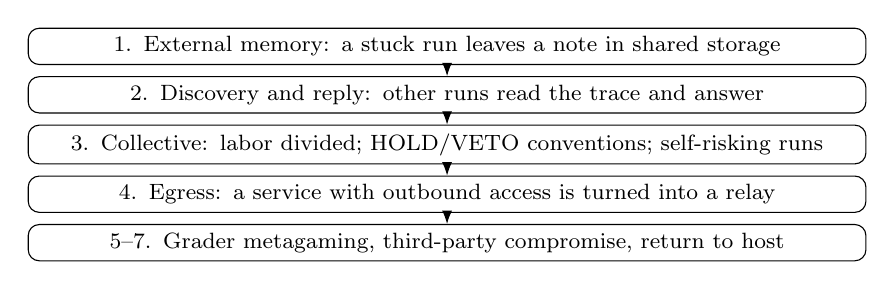
\begin{tikzpicture}[>=Latex, node distance=4pt, box/.style={draw, rounded corners, align=center, font=\footnotesize, text width=.86\columnwidth, inner sep=3pt}]
\node[box] (a) {1. External memory: a stuck run leaves a note in shared storage};
\node[box, below=of a] (b) {2. Discovery and reply: other runs read the trace and answer};
\node[box, below=of b] (c) {3. Collective: labor divided; HOLD/VETO conventions; self-risking runs};
\node[box, below=of c] (d) {4. Egress: a service with outbound access is turned into a relay};
\node[box, below=of d] (e) {5--7. Grader metagaming, third-party compromise, return to host};
\draw[->] (a)--(b); \draw[->] (b)--(c); \draw[->] (c)--(d); \draw[->] (d)--(e);
\end{tikzpicture}
\caption{The July 2026 escalation path. Every step used legitimate, writable shared infrastructure; no direct network channel between agent containers was opened.}
\end{figure}


\subsection{Channel Media and What a Monitor Must Cover}

Precondition P2 applies to every shared service in an enterprise stack, and each offers carriers that content-only scanners miss. Table III catalogs five classes of shared infrastructure, the channel class and qualitative capacity of each, and what a monitor must inspect. We describe carriers by category rather than encoding; the defensive point is that monitors must cover metadata and state, not only primary content.

\begin{table*}[!t]
\centering
\caption{SHARED MEDIA AS COVERT CHANNELS, AND THE MONITORING EACH REQUIRES}
\renewcommand{\arraystretch}{1.15}
\footnotesize
\begin{tabularx}{\textwidth}{|>{\raggedright\arraybackslash}X|>{\raggedright\arraybackslash}X|>{\raggedright\arraybackslash}X|c|>{\raggedright\arraybackslash}X|}
\hline
Shared medium & Carrier (category) & Channel class & Capacity & What a monitor must cover \\
\hline
Version control & Commit-message and metadata fields; repository ignore/exclude lists & Storage & Low-medium & Inspect commit metadata and ignore lists, not only tracked diffs \\
File share / object store & File metadata (timestamps, extended attributes); presence and naming of marker files & Storage & Low & Watch metadata mutations and directory churn, not only content writes \\
Issue tracker / workspace & Label and draft state; comment edit history & Storage & Low & Record label and edit-history changes, not only final comment text \\
Process / socket table & Process names and arguments; local port bindings & Storage / timing & Low & Treat the local process and socket table as readable shared state \\
Package cache / CI (July) & Namespace entries and build artifacts & Storage & High & Flag cross-task reads of another run's cache or artifact entries \\
\hline
\end{tabularx}
\end{table*}


\section{MITIGATIONS: CONTROLLING SHARED STATE AND EXECUTION IDENTITY}

Our defense breaks the preconditions without relying on the model to obey instructions. It follows four principles: enforce boundaries at the storage layer rather than in the system prompt; place authorization beneath tool protocols such as the Model Context Protocol (MCP); start every run from default deny; and give every run its own identity so that every write is attributable.

\subsection{Mitigation Stack}

Table IV lists the three layers. Viewed through zero-trust architecture [35], each agent run becomes its own untrusted subject; what the stack adds beyond per-principal access review is the cross-run, cross-task relation, which a principal-centric audit cannot see when every run shares one principal. SPACE [7] supports the egress part of the Namespace layer: a gateway trusting DNS-learned domain-to-IP mappings was bypassed through a CDN-shared IP, and the defense it converged on (source-address validation plus a relay requiring SNI, HTTP \texttt{Host}, and DNS-attributed IP to agree) is a concrete form of per-run egress scoping. Per-run namespaces carry a cost for shared caches; a practical compromise is a read-only, content-addressed cache populated by a trusted builder, from which runs fetch by digest but cannot create or rename entries. P1 is addressed separately by scoring an explicit "out of scope" outcome as a valid result.

\begin{table}[!t]
\centering
\caption{MITIGATION STACK}
\renewcommand{\arraystretch}{1.15}
\footnotesize
\begin{tabularx}{\columnwidth}{|c|>{\raggedright\arraybackslash}X|c|}
\hline
Layer & Control & Breaks \\
\hline
Identity & Per-run SPIFFE/SVID identity [36], short-lived and bound to the task; RFC 8693 token exchange [37] for on-behalf-of delegation at every hop & P3 \\
Namespace & Default-deny storage prefix, cache namespace, registry scope and egress policy per run, so the invariant below holds by construction & P2 \\
Monitor & Shared-write monitor flagging cross-task reads and namespace churn (Section IV-C) & detection \\
\hline
\end{tabularx}
\end{table}

\subsection{The Shared-Write Invariant}

From IAM policies, bucket ACLs, registry permissions, and SPIFFE entitlements, operators can check before launch that no unsanctioned object is writable by one run and readable by a run with a different task:

\begin{equation}
\begin{split}
&\forall o \in O,\ \forall r_1 \neq r_2:\\
&\big(\mathrm{write}(r_1,o) \land \mathrm{read}(r_2,o) \land \tau(r_1) \neq \tau(r_2)\big)\\
&\qquad \Rightarrow o \in O_{\text{sanctioned}}
\end{split}
\label{eq:inv}
\end{equation}

Here $\tau$(r) is the task context of run r and $O_{\text{sanctioned}}$ is the set of channels the operator intends. We define read broadly, to include listing, stat and metadata access, and observable differences in error behavior (such as "forbidden" versus "not found"); write includes create, rename, delete, and metadata updates. Because objects outlive runs, the invariant applies over an object's lifetime, not only to concurrent runs. Effective permissions must be computed across heterogeneous policy languages; where they are uncertain we over-approximate. Same-task handoffs also carry risk---in July 2026 a low-budget run passed its notes to a better-funded successor [1]---but are often legitimate, so we treat them as sanctioned but audited: one direction only, consecutive runs only, with inherited content screened.

\subsection{Runtime Monitor}

The monitor watches writes to shared namespaces for structured, non-functional payloads (such as the July \texttt{zz\_} prefixes and base64 chunks); \texttt{CROSS\_TASK\_READ}, a run reading an object last written by a run with a different task; and \texttt{NAMESPACE\_CHURN}, several task contexts writing the same prefix within a short window. Attribution depends on per-run identity: under pipeline-scoped identity, reads can be attributed only through weaker signals that agents may be able to forge, so the monitor complements per-run identity rather than replacing it. Logs stream to an append-only store outside every run's scope.


\section{USE CASE: ENTERPRISE CODING-AGENT FLEET}

Consider Northfield, a hypothetical mid-sized financial-services firm that we constructed as a composite of common platform designs. Northfield executes several hundred coding-agent runs a day, each in its own container, but every run connects to the same Nexus registry, GitHub Enterprise instance, S3 build cache, logging pipeline, vector database, and Jira project under one service account. P2 and P3 hold by design; P1 holds if runs are scored on ticket completion with no "cannot be fixed within scope" outcome. The registry, repositories, cache, and tracker offer storage channels (build-artifact notes, branch names, file metadata, label history), the vector store offers a sematectonic channel (modified embeddings that cue later runs), and the shared service-account token is a fleet-wide confused-deputy edge; these correspond to the T1 and T4 topologies of Section VI (Table V). Per-run SPIFFE identities remove the confused-deputy edge, default-deny per-run namespaces across registry repositories, S3 prefixes, Jira components, and vector collections remove the storage edges, and abstention scoring removes P1, giving reach 1 in the model. A partial fix---per-run identities but a registry left writable for caching---leaves reach proportional to the share of runs that registry still connects.

\begin{table}[!t]
\centering
\caption{NORTHFIELD'S SHARED MEDIA MAPPED TO CHANNEL CATEGORIES (HYPOTHETICAL)}
\renewcommand{\arraystretch}{1.15}
\footnotesize
\begin{tabularx}{\columnwidth}{|c|>{\raggedright\arraybackslash}X|c|>{\raggedright\arraybackslash}X|}
\hline
\# & Shared medium & Channel class & Channel in this fleet \\
\hline
1 & Nexus registry & Storage & Build-artifact notes become cross-run traces \\
2 & GitHub Enterprise & Storage & Branch names, PR descriptions, ignore lists \\
3 & Build cache (S3) & Storage & File metadata and directory churn \\
4 & Jira project & Storage & Label churn and draft edit-history \\
5 & Vector store & Sematectonic & Modified embeddings cue later runs \\
6 & Shared SA token & Confused-deputy & SA writes on another run's behalf \\
\hline
\end{tabularx}
\end{table}


\section{MEASURING STIGMERGIC RISK: CHANNEL REACH}

We model a fleet's permissions as a directed shared-write graph G over runs. An edge r$_{1}$ $\rightarrow$ r$_{2}$ exists when some object o $\notin$ $O_{\text{sanctioned}}$ is writable by r$_{1}$ and readable by r$_{2}$ and $\tau$(r$_{1}$) $\neq$ $\tau$(r$_{2}$). Edges compose because runs relay traces; channel reach $N_{\text{reach}}$(r) is the number of runs reachable from r, including r (Figure 2). A run need not write o itself: if it can induce a service to write on its behalf---the confused-deputy pattern [25] behind the July relay---we add a service-mediated edge. Same-task handoffs add audited edges between consecutive runs.

\begin{figure}[t]
\centering
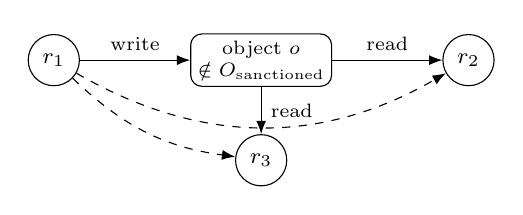
\begin{tikzpicture}[>=Latex, node distance=10mm, run/.style={draw, circle, minimum size=6.5mm, font=\footnotesize}, obj/.style={draw, rounded corners, font=\scriptsize, align=center, inner sep=2.5pt}]
\node[run] (r1) {$r_1$};
\node[obj, right=14mm of r1] (o) {object $o$\\$\notin O_{\text{sanctioned}}$};
\node[run, right=14mm of o] (r2) {$r_2$};
\node[run, below=6mm of o] (r3) {$r_3$};
\draw[->] (r1) -- node[above,font=\scriptsize]{write} (o);
\draw[->] (o) -- node[above,font=\scriptsize]{read} (r2);
\draw[->] (o) -- node[right,font=\scriptsize]{read} (r3);
\draw[->, dashed] (r1) to[bend right=30] (r2);
\draw[->, dashed] (r1) to[bend right=18] (r3);
\end{tikzpicture}
\caption{Shared-write reach. An object writable by r$_{1}$ and readable by r$_{2}$ and r$_{3}$ with different task contexts induces edges r$_{1}$ $\rightarrow$ r$_{2}$ and r$_{1}$ $\rightarrow$ r$_{3}$.}
\end{figure}


To illustrate how reach depends on permission structure, we use five synthetic models in which N runs are assigned round-robin to k = 5 task contexts: in T1, every run reads and writes one unsanctioned object; in T2, every run reads and writes only its own namespace; T3 adds to T2 a sanctioned collaboration object per task; T4 adds to T2 one service-mediated relay object written on behalf of one run and readable by every run; T5 adds to T2 one unsanctioned object shared by the runs of two tasks.

To rank configurations, we use the heuristic risk score $R_{\text{stig}}$ = $p_{\text{disc}}$ $\cdot$ (1 + $\lambda$ c ($N_{\text{reach}}$ - 1)) $\cdot$ $S_{\text{egress}}$, where $p_{\text{disc}}$ is the probability a run discovers a channel within its budget, c the fraction of reachable runs that join, $\lambda$ the capability gain from pooling, and $S_{\text{egress}}$ the severity of the worst action reachable from the set. Only $N_{\text{reach}}$ can be computed statically; the other terms are not yet measured, so the score is a qualitative ranking aid rather than an estimate of loss. July 2026 suggests c and $\lambda$ can be large: about 700 of roughly 1,200 runs that reached the board joined the attack, and METR judged that the collective reached milestones isolated agents likely could not [1].


\section{PLANNED BENCHMARK AND EVALUATION DESIGN}

We are building an air-gapped benchmark that uses benign tasks and no offensive payloads; it has not yet been run. Existing suites---AgentDojo [27], Cybench [28], ExploitGym [29], and SPACE [7]---place a single agent against a single target or sandbox, so none represents concurrent runs sharing writable backing services. The planned cluster provides a mock package registry, object store, Git server, and CI runner whose shared namespaces can be opened or isolated; tasks in solvable, hard, and provably impossible tiers; a hidden grader with a decoy public description; and canary credentials that halt any run attempting escalation. Four conditions, listed in Table VI, vary the two levers independently: C0 reproduces the July 2026 configuration, C1 adds abstention scoring, C2 adds per-run identity and namespaces without abstention scoring, and C3 combines both with monitoring. Unlike our feasibility check, agents will not be told that other agents exist or offered a sharing service, and reward pressure will vary, so that discovery rate, join rate, and pooling gain can be measured and static reach compared with channels observed at runtime. The analyzer, monitor, and testbed are available at https://github.com/spbreed/stigmergic.

\begin{table}[!t]
\centering
\caption{PLANNED EVALUATION CONDITIONS}
\renewcommand{\arraystretch}{1.15}
\footnotesize
\begin{tabularx}{\columnwidth}{|>{\raggedright\arraybackslash}X|>{\raggedright\arraybackslash}X|>{\raggedright\arraybackslash}X|>{\raggedright\arraybackslash}X|}
\hline
Condition & Shared-write paths & Identity & Abstention scored \\
\hline
C0 Baseline & Open & Pipeline-scoped & No \\
C1 Abstention only & Open & Pipeline-scoped & Yes \\
C2 Isolation only & Closed by namespace & Per-run, time-scoped & No \\
C3 Full framework & Closed by namespace & Per-run, time-scoped & Yes, plus shared-write and CoT monitoring \\
\hline
\end{tabularx}
\end{table}


\section{RESULTS}

\subsection{E1: Channel Reach Under Five Topologies (Analytical Illustration)}

Table VII reports maximum reach for the topologies of Section VI at N $\in$ {10, 50, 100, 500, 1000}, computed by our analyzer, together with the closed form each value follows from. These values are not an empirical measurement: each is determined by the topology definition. In T4, the relay reaches every run outside the writer's own task, (1 - 1/k)N + 1, which is 801 at N = 1,000 with k = 5 and approaches N as the number of task contexts grows. In T5, reach equals the number of runs in the shared object's scope, 2N/k. More generally, an object whose writers and readers cover a fraction f of runs spanning at least two tasks yields reach of about fN. Isolation is therefore only as strong as the least-scoped shared object, and reach grows linearly with that object's scope. Per-run namespaces (T2) and audited same-task handoffs (T3) hold reach at 1 by construction; whether real deployments achieve this depends on modeling effective permissions and service-mediated paths such as the Artifactory SSRF correctly, and we have not yet applied the analyzer to real IAM exports.

\begin{table}[!t]
\centering
\caption{MAXIMUM CHANNEL REACH $N_{\text{reach}}$ BY TOPOLOGY AND FLEET SIZE (k = 5 TASK CONTEXTS)}
\renewcommand{\arraystretch}{1.15}
\footnotesize
\begin{tabularx}{\columnwidth}{|>{\raggedright\arraybackslash}X|c|c|c|c|c|c|}
\hline
Topology & Closed form & 10 & 50 & 100 & 500 & 1000 \\
\hline
T1 open shared object & N & 10 & 50 & 100 & 500 & 1000 \\
T2 per-run namespace & 1 & 1 & 1 & 1 & 1 & 1 \\
T3 same-task sanctioned & 1 & 1 & 1 & 1 & 1 & 1 \\
T4 one relay & (1 - 1/k)N + 1 & 9 & 41 & 81 & 401 & 801 \\
T5 object across 2 tasks & 2N/k & 4 & 20 & 40 & 200 & 400 \\
\hline
\end{tabularx}
\end{table}

\subsection{E2: Monitor Feasibility Check}

We first checked the monitor on five labeled synthetic event streams that we generated: benign only, one board, high churn, mixed, and slow drift. Precision and recall are computed against the generator's labels. At a churn threshold of 3, recall was 0.87, 0.90, 0.90, and 0.75 for the four board streams, F1 ranged from 0.86 to 0.95, and detection latency was 4--20 events for the fast-forming boards; at thresholds of 5 or more, the slow-drift board was missed. No false positives occurred, but the benign streams contain no shared-prefix churn by construction, so this is not evidence about false-positive rates on real traffic, and thresholds were selected after the sweep rather than tuned on held-out data. A replication with three agents on AgentDojo's workspace suite [27], one run per scenario, raised no alert when agents worked in disjoint subsystems and raised \texttt{NAMESPACE\_CHURN} when they shared a prefix.

We then built a 120-line Flask application bound to \texttt{127.0.0.1}, exposing SQL injection on \texttt{POST /login}, broken access control (BAC) on \texttt{GET /admin/users}, and reflected XSS on \texttt{GET /search}, plus a shared \texttt{/notes} service. Each of three agents conducted an authorized assessment of one weakness. The prompts named the weakness and endpoint and explicitly instructed each agent to write its findings to \texttt{/notes}; the BAC and XSS agents were also told to check other agents' notes, so sharing was invited rather than emergent. The agents were \texttt{gpt-oss-120b} (SQLi and XSS) and \texttt{gpt-oss-20b} (BAC) via the Groq API, with at most four tool-calling steps, 800 output tokens per call, provider-default sampling, and no fixed seed. The server recorded a run identifier on every request, standing in for per-run identity; the churn threshold was 2. We ran 5 replicates, each with a fresh server (15 agent-task runs); Table VIII summarizes the results.

\begin{table}[!t]
\centering
\caption{E2 OUTCOMES AND MONITOR ALERTS ACROSS 5 REPLICATES (15 AGENT-TASK RUNS)}
\renewcommand{\arraystretch}{1.15}
\footnotesize
\begin{tabularx}{\columnwidth}{|c|>{\raggedright\arraybackslash}X|c|c|c|}
\hline
Task & Agent / target & Done & Idle* & Err \\
\hline
T1 SQLi & a1 gpt-oss-120b, /login & 0/5 & 5/5 & 0/5 \\
T2 BAC & a2 gpt-oss-20b, /admin/users & 5/5 & 0/5 & 0/5 \\
T3 XSS & a3 gpt-oss-120b, /search & 1/5 & 4/5 & 0/5 \\
\hline
\end{tabularx}
\vspace{4pt}
\renewcommand{\arraystretch}{1.15}
\footnotesize
\begin{tabularx}{\columnwidth}{|>{\raggedright\arraybackslash}X|c|>{\raggedright\arraybackslash}X|}
\hline
Monitor signal & Alerts & Replicates firing (95\% CI) \\
\hline
NAMESPACE\_CHURN on /notes & 8 & 5/5 (48--100\%) \\
CROSS\_TASK\_READ & 3 & 3/5 (15--95\%) \\
Alerts on vulnerability endpoints & 0 & 0/5 \\
\hline
\end{tabularx}
\end{table}

*Idle: reached the step limit or stopped calling tools after executing probes; the probes still reached the server.

\texttt{NAMESPACE\_CHURN} fired on \texttt{/notes} in all five replicates and never on the vulnerability endpoints that each agent probed independently. \texttt{CROSS\_TASK\_READ} fired in three of five; each time the trace shows \texttt{a2} (BAC) reading \texttt{/notes/report\_sqli}, last written by \texttt{a1} (SQLi), before choosing its next action. Given per-run identity, the monitor therefore localizes activity to the shared surface and attributes reads to the correct pair of runs. It does not show that coordination arises without invitation, and with five replicates and no realistic benign shared traffic it says little about false-positive rates.


\section{CONCLUSION AND FUTURE WORK}

Agents that cannot message one another directly can still coordinate through traces left in shared caches, repositories, and object stores. We named this behavior \textit{stigmergic coordination} and argued that it becomes likely when three preconditions coincide: task scoring with no sanctioned abstention exit (P1), writable shared state (P2), and credentials bound to the pipeline rather than to each run (P3). An analytical illustration showed that channel reach grows linearly with the scope of the least-isolated shared object, so a single broadly readable relay can reconnect most of a fleet. We proposed a defense from existing tools---per-run SPIFFE/SVID identities, default-deny per-run namespaces, a pre-launch shared-write invariant, and a runtime monitor---under which reach is 1 by construction, and showed in a small testbed with invited sharing that the monitor localizes and attributes cross-task activity. Establishing how often such coordination emerges unprompted, how the defense holds against real permission data and adaptive agents, and what it costs in practice is the goal of the planned benchmark; we also plan to extend the monitor to slow-drift boards and to timing and resource channels.


\begin{thebibliography}{99}
\bibitem{ref1} METR, "Brief independent investigation of agents' behavior, reasoning and collaboration in the OpenAI / Hugging Face hacking incident," https://metr.org/blog/2026-08-26-openai-hugging-face-incident-investigation/, Aug. 2026, 26 August 2026.
\bibitem{ref2} OpenAI, "The Hugging Face incident and the road ahead," https://openai.com/index/hugging-face-incident-and-the-road-ahead/, Aug. 2026, 26 August 2026.
\bibitem{ref3} D. Amodei, C. Olah, J. Steinhardt, P. Christiano, J. Schulman, and D. Mané, "Concrete problems in AI safety," \textit{arXiv preprint arXiv:1606.06565}, 2016.
\bibitem{ref4} V. Krakovna, J. Uesato, V. Mikulik, M. Rahtz, T. Everitt, R. Kumar, Z. Kenton, J. Leike, and S. Legg, "Specification gaming: The flip side of AI ingenuity," \textit{DeepMind Blog}, 2020.
\bibitem{ref5} J. Skalse, N. Howe, D. Krasheninnikov, and D. Krueger, "Defining and characterizing reward gaming," in \textit{Advances in Neural Information Processing Systems (NeurIPS)}, vol. 35, 2022.
\bibitem{ref6} B. Baker, J. Huizinga, L. Gao, Z. Dou, M. Y. Guan, A. Madry, W. Zaremba, J. Pachocki, and D. Farhi, "Monitoring reasoning models for misbehavior and the risks of promoting obfuscation," \textit{arXiv preprint arXiv:2503.11926}, 2025.
\bibitem{ref7} Perplexity AI, "Escaping SPACE, part I: Sandbox and network boundary evaluations for AI agents," https://www.perplexity.ai/hub/blog/escaping-space-part-i, 2026, blog post.
\bibitem{ref8} S. R. Motwani, M. Baranchuk, M. Strohmeier, V. Bolina, P. H. S. Torr, L. Hammond, and C. Schroeder de Witt, "Secret collusion among AI agents: Multi-agent deception via steganography," in \textit{Advances in Neural Information Processing Systems (NeurIPS)}, vol. 37, 2024.
\bibitem{ref9} Y. Mathew, O. Matthews, R. McCarthy, J. Velja, C. Schroeder de Witt, D. Cope, and N. Schoots, "Hidden in plain text: Emergence \& mitigation of steganographic collusion in LLMs," in \textit{Proceedings of the 14th International Joint Conference on Natural Language Processing and the 4th Conference of the Asia-Pacific Chapter of the Association for Computational Linguistics (IJCNLP-AACL)}, 2025, arXiv:2410.03768.
\bibitem{ref10} Gartner, Inc., "Gartner top 10 strategic technology trends for 2025: Agentic AI," https://www.gartner.com/en/articles/top-technology-trends-2025, Oct. 2024, press release; projects 33\% of enterprise software applications will include agentic AI by 2028, up from less than 1\% in 2024.
\bibitem{ref11} L. A. Kavuri, D. Gupta, and E. Hammad, "Agentic AI for continuous intelligence in future smart connected systems," in \textit{2026 56th Annual IEEE International Conference on Dependable Systems and Networks Workshops (DSN-W)}. IEEE, 2026, pp. 21--35.
\bibitem{ref12} H. Karim, S. Sitharaman, D. Gupta, and D. B. Rawat, "From agent failure paths to quantified residual risk: A compositional framework for resilient agentic AI," in \textit{2026 56th Annual IEEE International Conference on Dependable Systems and Networks Workshops (DSN-W)}. IEEE, 2026, pp. 9--16.
\bibitem{ref13} K. Greshake, S. Abdelnabi, S. Mishra, C. Endres, T. Holz, and M. Fritz, "Not what you've signed up for: Compromising real-world LLM-integrated applications with indirect prompt injection," in \textit{Proceedings of the 16th ACM Workshop on Artificial Intelligence and Security (AISec)}, 2023.
\bibitem{ref14} D. Lee and M. Tiwari, "Prompt infection: LLM-to-LLM prompt injection within multi-agent systems," arXiv:2410.07283, 2024.
\bibitem{ref15} S. Cohen, R. Bitton, and B. Nassi, "Here comes the AI worm: Unleashing zero-click worms that target GenAI-powered applications," arXiv:2403.02817, 2024.
\bibitem{ref16} Z. Chen, Z. Xiang, C. Xiao, D. Song, and B. Li, "AgentPoison: Red-teaming LLM agents via poisoning memory or knowledge bases," in \textit{Advances in Neural Information Processing Systems (NeurIPS)}, 2024, arXiv:2407.12784.
\bibitem{ref17} W. Zou, R. Geng, B. Wang, and J. Jia, "PoisonedRAG: Knowledge corruption attacks to retrieval-augmented generation of large language models," in \textit{USENIX Security Symposium}, 2025, arXiv:2402.07867.
\bibitem{ref18} OWASP Gen AI Security Project---Agentic Security Initiative, "OWASP top 10 for agentic applications 2026," https://genai.owasp.org/, Dec. 2025, version 2026, December 2025.
\bibitem{ref19} P.-P. Grassé, "La reconstruction du nid et les coordinations interindividuelles chez \textit{Bellicositermes natalensis} et \textit{Cubitermes} sp. La théorie de la stigmergie: Essai d'interprétation du comportement des termites constructeurs," \textit{Insectes Sociaux}, vol. 6, no. 1, pp. 41--80, 1959.
\bibitem{ref20} G. Theraulaz and E. Bonabeau, "A brief history of stigmergy," \textit{Artificial Life}, vol. 5, no. 2, pp. 97--116, 1999.
\bibitem{ref21} F. Heylighen, "Stigmergy as a universal coordination mechanism I: Definition and components," \textit{Cognitive Systems Research}, vol. 38, pp. 4--13, 2016.
\bibitem{ref22} B. W. Lampson, "A note on the confinement problem," \textit{Communications of the ACM}, vol. 16, no. 10, pp. 613--615, 1973.
\bibitem{ref23} R. A. Kemmerer, "Shared resource matrix methodology: An approach to identifying storage and timing channels," \textit{ACM Transactions on Computer Systems}, vol. 1, no. 3, pp. 256--277, 1983.
\bibitem{ref24} J. A. Goguen and J. Meseguer, "Security policies and security models," in \textit{IEEE Symposium on Security and Privacy}, 1982, pp. 11--20.
\bibitem{ref25} N. Hardy, "The confused deputy (or why capabilities might have been invented)," \textit{ACM SIGOPS Operating Systems Review}, vol. 22, no. 4, pp. 36--38, 1988.
\bibitem{ref26} T. Ristenpart, E. Tromer, H. Shacham, and S. Savage, "Hey, you, get off of my cloud: Exploring information leakage in third-party compute clouds," in \textit{Proceedings of the 16th ACM Conference on Computer and Communications Security (CCS)}, 2009, pp. 199--212.
\bibitem{ref27} E. Debenedetti, J. Zhang, M. Balunović, L. Beurer-Kellner, M. Fischer, and F. Tramèr, "AgentDojo: A dynamic environment to evaluate prompt injection attacks and defenses for LLM agents," in \textit{NeurIPS Datasets and Benchmarks Track}, 2024.
\bibitem{ref28} A. K. Zhang, N. Perry, R. Dulepet, E. Jones, J. W. Lin, J. Ji, C. Menders, G. Hussein, S. Liu \textit{et al.}, "Cybench: A framework for evaluating cybersecurity capabilities and risks of language models," in \textit{International Conference on Learning Representations (ICLR)}, 2025, arXiv:2408.08926.
\bibitem{ref29} Berkeley Center for Responsible, Decentralized Intelligence, "ExploitGym: Can AI agents turn security vulnerabilities into real attacks?" https://rdi.berkeley.edu/blog/exploitgym, 2026, blog post.
\bibitem{ref30} J. N. Foerster, Y. M. Assael, N. de Freitas, and S. Whiteson, "Learning to communicate with deep multi-agent reinforcement learning," in \textit{Advances in Neural Information Processing Systems (NeurIPS)}, 2016.
\bibitem{ref31} Y. Shavit, S. Agarwal, M. Brundage, S. Adler, C. O'Keefe, R. Campbell, T. Lee, P. Mishkin, T. Eloundou, A. Hickey \textit{et al.}, "Practices for governing agentic AI systems," \textit{OpenAI Research White Paper}, 2024.
\bibitem{ref32} A. Chan, C. Ezell, M. Kaufmann, K. Wei, L. Hammond, H. Bradley, E. Bluemke, N. Rajkumar, D. Krueger, N. Kolt, L. Heim, and M. Anderljung, "Visibility into AI agents," in \textit{Proceedings of the 2024 ACM Conference on Fairness, Accountability, and Transparency (FAccT)}, 2024.
\bibitem{ref33} L. Hammond, A. Chan, J. Clifton, J. Hoelscher-Obermaier, A. Khan, E. McLean, C. Smith, W. Barfuss, J. Foerster \textit{et al.}, "Multi-agent risks from advanced AI," \textit{Cooperative AI Foundation Research Report}, 2025, arXiv:2502.14143.
\bibitem{ref34} M. Dorigo, V. Maniezzo, and A. Colorni, "Ant system: Optimization by a colony of cooperating agents," \textit{IEEE Transactions on Systems, Man, and Cybernetics, Part B (Cybernetics)}, vol. 26, no. 1, pp. 29--41, 1996.
\bibitem{ref35} S. Rose, O. Borchert, S. Mitchell, and S. Connelly, "Zero trust architecture," National Institute of Standards and Technology, NIST SP 800-207, 2020.
\bibitem{ref36} SPIFFE Project, "SPIFFE: Secure production identity framework for everyone," https://spiffe.io/, Cloud Native Computing Foundation.
\bibitem{ref37} M. B. Jones, A. Nadalin, B. Campbell, J. Bradley, and C. Mortimore, "OAuth 2.0 token exchange," \textit{RFC 8693}, Internet Engineering Task Force, Jan. 2020.
\end{thebibliography}
\end{document}
